\documentclass{standalone}
\usepackage{tikz}
\usetikzlibrary{patterns, positioning}


\begin{document}
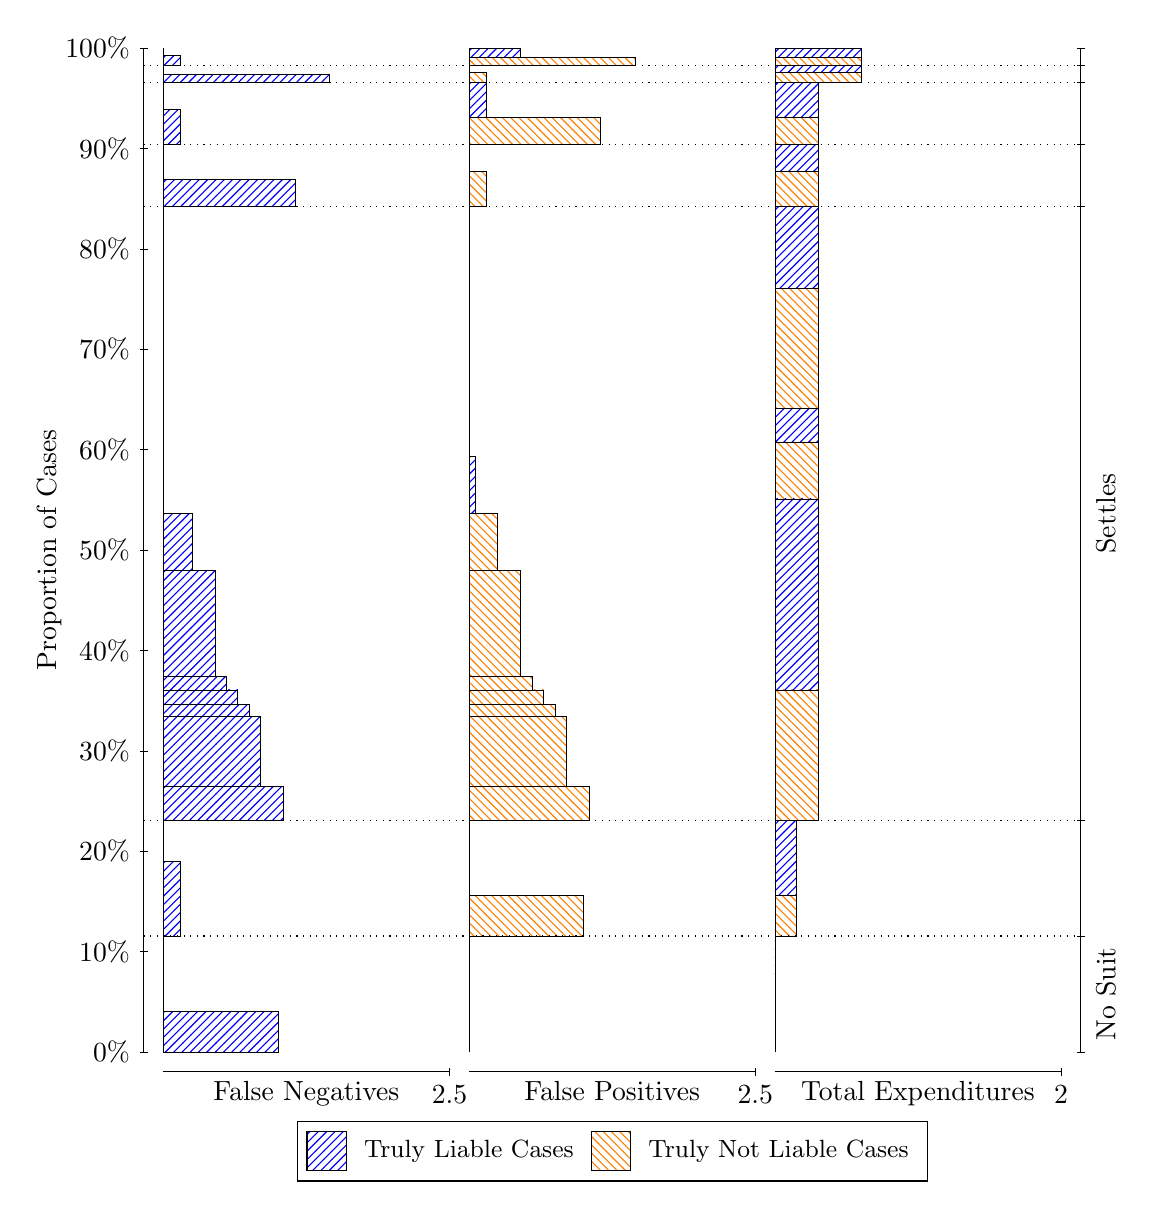
\begin{tikzpicture}
\draw[black, very thin] (1.5,1.75) -- (1.5,14.5);
\node[rotate=90, text=black, anchor=center] at (0.3, 8.125) {Proportion of Cases};
\draw[black, very thin] (1.45,1.75) -- (1.55,1.75);
\node[text=black, anchor=east] at (1.45, 1.75) {0\%};
\draw[black, very thin] (1.45,3.025) -- (1.55,3.025);
\node[text=black, anchor=east] at (1.45, 3.025) {10\%};
\draw[black, very thin] (1.45,4.3) -- (1.55,4.3);
\node[text=black, anchor=east] at (1.45, 4.3) {20\%};
\draw[black, very thin] (1.45,5.575) -- (1.55,5.575);
\node[text=black, anchor=east] at (1.45, 5.575) {30\%};
\draw[black, very thin] (1.45,6.85) -- (1.55,6.85);
\node[text=black, anchor=east] at (1.45, 6.85) {40\%};
\draw[black, very thin] (1.45,8.125) -- (1.55,8.125);
\node[text=black, anchor=east] at (1.45, 8.125) {50\%};
\draw[black, very thin] (1.45,9.4) -- (1.55,9.4);
\node[text=black, anchor=east] at (1.45, 9.4) {60\%};
\draw[black, very thin] (1.45,10.675) -- (1.55,10.675);
\node[text=black, anchor=east] at (1.45, 10.675) {70\%};
\draw[black, very thin] (1.45,11.95) -- (1.55,11.95);
\node[text=black, anchor=east] at (1.45, 11.95) {80\%};
\draw[black, very thin] (1.45,13.225) -- (1.55,13.225);
\node[text=black, anchor=east] at (1.45, 13.225) {90\%};
\draw[black, very thin] (1.45,14.5) -- (1.55,14.5);
\node[text=black, anchor=east] at (1.45, 14.5) {100\%};

\draw[black, very thin] (13.4,1.75) -- (13.4,14.5);
\draw[black, very thin] (13.35,1.75) -- (13.45,1.75);
\node[anchor=west] at (13.35, 1.75) {};
\draw[black, very thin] (13.35,3.2226) -- (13.45,3.2226);
\node[anchor=west] at (13.35, 3.2226) {};
\draw[black, very thin] (13.35,4.6887) -- (13.45,4.6887);
\node[anchor=west] at (13.35, 4.6887) {};
\draw[black, very thin] (13.35,12.492) -- (13.45,12.492);
\node[anchor=west] at (13.35, 12.492) {};
\draw[black, very thin] (13.35,13.28) -- (13.45,13.28);
\node[anchor=west] at (13.35, 13.28) {};
\draw[black, very thin] (13.35,14.067) -- (13.45,14.067);
\node[anchor=west] at (13.35, 14.067) {};
\draw[black, very thin] (13.35,14.283) -- (13.45,14.283);
\node[anchor=west] at (13.35, 14.283) {};
\draw[black, very thin] (13.35,14.5) -- (13.45,14.5);
\node[anchor=west] at (13.35, 14.5) {};

\draw[black, very thin, pattern color=blue, pattern=north east lines] (1.75,1.75) rectangle (3.2033,2.269);
\draw[black, very thin, pattern color=orange, pattern=north west lines] (1.75,2.269) rectangle (1.75,3.2226);
\draw[black, very thin, pattern color=blue, pattern=north east lines] (1.75,3.2226) rectangle (1.968,4.173);
\draw[black, very thin, pattern color=orange, pattern=north west lines] (1.75,4.173) rectangle (1.75,4.6887);
\draw[black, very thin, pattern color=blue, pattern=north east lines] (1.75,4.6887) rectangle (3.276,5.1189);
\draw[black, very thin, pattern color=blue, pattern=north east lines] (1.75,5.1189) rectangle (2.9853,6.0072);
\draw[black, very thin, pattern color=blue, pattern=north east lines] (1.75,6.0072) rectangle (2.84,6.1642);
\draw[black, very thin, pattern color=blue, pattern=north east lines] (1.75,6.1642) rectangle (2.6947,6.3473);
\draw[black, very thin, pattern color=blue, pattern=north east lines] (1.75,6.3473) rectangle (2.5493,6.5227);
\draw[black, very thin, pattern color=blue, pattern=north east lines] (1.75,6.5227) rectangle (2.404,7.8661);
\draw[black, very thin, pattern color=blue, pattern=north east lines] (1.75,7.8661) rectangle (2.1133,8.5906);
\draw[black, very thin, pattern color=orange, pattern=north west lines] (1.75,8.5906) rectangle (1.75,12.492);
\draw[black, very thin, pattern color=blue, pattern=north east lines] (1.75,12.492) rectangle (3.4213,12.834);
\draw[black, very thin, pattern color=orange, pattern=north west lines] (1.75,12.834) rectangle (1.75,13.28);
\draw[black, very thin, pattern color=blue, pattern=north east lines] (1.75,13.28) rectangle (1.968,13.725);
\draw[black, very thin, pattern color=orange, pattern=north west lines] (1.75,13.725) rectangle (1.75,14.067);
\draw[black, very thin, pattern color=blue, pattern=north east lines] (1.75,14.067) rectangle (3.8573,14.165);
\draw[black, very thin, pattern color=orange, pattern=north west lines] (1.75,14.165) rectangle (1.75,14.283);
\draw[black, very thin, pattern color=blue, pattern=north east lines] (1.75,14.283) rectangle (1.968,14.402);
\draw[black, very thin, pattern color=orange, pattern=north west lines] (1.75,14.402) rectangle (1.75,14.5);
\draw[black, very thin, pattern color=orange, pattern=north west lines] (5.6333,1.75) rectangle (5.6333,2.7036);
\draw[black, very thin, pattern color=blue, pattern=north east lines] (5.6333,2.7036) rectangle (5.6333,3.2226);
\draw[black, very thin, pattern color=orange, pattern=north west lines] (5.6333,3.2226) rectangle (7.0867,3.7383);
\draw[black, very thin, pattern color=blue, pattern=north east lines] (5.6333,3.7383) rectangle (5.6333,4.6887);
\draw[black, very thin, pattern color=orange, pattern=north west lines] (5.6333,4.6887) rectangle (7.1593,5.1189);
\draw[black, very thin, pattern color=orange, pattern=north west lines] (5.6333,5.1189) rectangle (6.8687,6.0071);
\draw[black, very thin, pattern color=orange, pattern=north west lines] (5.6333,6.0071) rectangle (6.7233,6.1642);
\draw[black, very thin, pattern color=orange, pattern=north west lines] (5.6333,6.1642) rectangle (6.578,6.3473);
\draw[black, very thin, pattern color=orange, pattern=north west lines] (5.6333,6.3473) rectangle (6.4327,6.5227);
\draw[black, very thin, pattern color=orange, pattern=north west lines] (5.6333,6.5227) rectangle (6.2873,7.8661);
\draw[black, very thin, pattern color=orange, pattern=north west lines] (5.6333,7.8661) rectangle (5.9967,8.5906);
\draw[black, very thin, pattern color=blue, pattern=north east lines] (5.6333,8.5906) rectangle (5.706,9.3151);
\draw[black, very thin, pattern color=blue, pattern=north east lines] (5.6333,9.3151) rectangle (5.6333,12.492);
\draw[black, very thin, pattern color=orange, pattern=north west lines] (5.6333,12.492) rectangle (5.8513,12.938);
\draw[black, very thin, pattern color=blue, pattern=north east lines] (5.6333,12.938) rectangle (5.6333,13.28);
\draw[black, very thin, pattern color=orange, pattern=north west lines] (5.6333,13.28) rectangle (7.3047,13.621);
\draw[black, very thin, pattern color=blue, pattern=north east lines] (5.6333,13.621) rectangle (5.8513,14.067);
\draw[black, very thin, pattern color=orange, pattern=north west lines] (5.6333,14.067) rectangle (5.8513,14.186);
\draw[black, very thin, pattern color=blue, pattern=north east lines] (5.6333,14.186) rectangle (5.6333,14.283);
\draw[black, very thin, pattern color=orange, pattern=north west lines] (5.6333,14.283) rectangle (7.7407,14.381);
\draw[black, very thin, pattern color=blue, pattern=north east lines] (5.6333,14.381) rectangle (6.2873,14.5);
\draw[black, very thin, pattern color=orange, pattern=north west lines] (9.5167,1.75) rectangle (9.5167,2.7036);
\draw[black, very thin, pattern color=blue, pattern=north east lines] (9.5167,2.7036) rectangle (9.5167,3.2226);
\draw[black, very thin, pattern color=orange, pattern=north west lines] (9.5167,3.2226) rectangle (9.7892,3.7383);
\draw[black, very thin, pattern color=blue, pattern=north east lines] (9.5167,3.7383) rectangle (9.7892,4.6887);
\draw[black, very thin, pattern color=orange, pattern=north west lines] (9.5167,4.6887) rectangle (10.062,6.3473);
\draw[black, very thin, pattern color=blue, pattern=north east lines] (9.5167,6.3473) rectangle (10.062,8.7736);
\draw[black, very thin, pattern color=orange, pattern=north west lines] (9.5167,8.7736) rectangle (10.062,9.4981);
\draw[black, very thin, pattern color=blue, pattern=north east lines] (9.5167,9.4981) rectangle (10.062,9.9284);
\draw[black, very thin, pattern color=orange, pattern=north west lines] (9.5167,9.9284) rectangle (10.062,11.447);
\draw[black, very thin, pattern color=blue, pattern=north east lines] (9.5167,11.447) rectangle (10.062,12.492);
\draw[black, very thin, pattern color=orange, pattern=north west lines] (9.5167,12.492) rectangle (10.062,12.938);
\draw[black, very thin, pattern color=blue, pattern=north east lines] (9.5167,12.938) rectangle (10.062,13.28);
\draw[black, very thin, pattern color=orange, pattern=north west lines] (9.5167,13.28) rectangle (10.062,13.621);
\draw[black, very thin, pattern color=blue, pattern=north east lines] (9.5167,13.621) rectangle (10.062,14.067);
\draw[black, very thin, pattern color=orange, pattern=north west lines] (9.5167,14.067) rectangle (10.607,14.186);
\draw[black, very thin, pattern color=blue, pattern=north east lines] (9.5167,14.186) rectangle (10.607,14.283);
\draw[black, very thin, pattern color=orange, pattern=north west lines] (9.5167,14.283) rectangle (10.607,14.381);
\draw[black, very thin, pattern color=blue, pattern=north east lines] (9.5167,14.381) rectangle (10.607,14.5);
\draw[black, dotted] (1.5,3.2226) -- (13.4,3.2226);
\draw[black, dotted] (1.5,4.6887) -- (13.4,4.6887);
\draw[black, dotted] (1.5,12.492) -- (13.4,12.492);
\draw[black, dotted] (1.5,13.28) -- (13.4,13.28);
\draw[black, dotted] (1.5,14.067) -- (13.4,14.067);
\draw[black, dotted] (1.5,14.283) -- (13.4,14.283);
\draw[black, very thin] (1.75,1.5) -- (5.3833,1.5);
\node[text=black, anchor=north] at (3.5667, 1.5) {False Negatives};
\draw[black, very thin] (5.3833,1.45) -- (5.3833,1.55);
\node[text=black, anchor=north] at (5.3833, 1.45) {2.5};

\draw[black, very thin] (5.6333,1.5) -- (9.2667,1.5);
\node[text=black, anchor=north] at (7.45, 1.5) {False Positives};
\draw[black, very thin] (9.2667,1.45) -- (9.2667,1.55);
\node[text=black, anchor=north] at (9.2667, 1.45) {2.5};

\draw[black, very thin] (9.5167,1.5) -- (13.15,1.5);
\node[text=black, anchor=north] at (11.333, 1.5) {Total Expenditures};
\draw[black, very thin] (13.15,1.45) -- (13.15,1.55);
\node[text=black, anchor=north] at (13.15, 1.45) {2};

\node[text=black, centered, rotate=90] at (13.72, 2.4863) {No Suit};

\node[text=black, centered, rotate=90] at (13.72, 8.5906) {Settles};





\draw (7.449999999999999,1.5) node[draw=none] (baseCoordinate) {};
\begin{scope}[align=center]
        \matrix[scale=0.5, draw=black, below=0.5cm of baseCoordinate, nodes={draw}, column sep=0.1cm]{
            \node[rectangle, draw, minimum width=0.5cm, minimum height=0.5cm, pattern color=blue, pattern=north east lines] {}; &
            \node[draw=none, font=\small, text=black] (B) {Truly Liable Cases}; &
            \node[rectangle, draw, minimum width=0.5cm, minimum height=0.5cm, pattern color=orange, pattern=north west lines] {}; &
            \node[draw=none, font=\small, text=black] (B) {Truly Not Liable Cases}; \\
            };
\end{scope}

\end{tikzpicture}
\end{document}